\par
Figure~\ref{fig:additional-annotation-examples} illustrates further type and boundary decisions. Panel (a) assigns T to conversational ability, service awareness, interpersonal communication, and coordination. Panel (b) retains the historical S spans for presales consulting, project management, and presales work on large projects. The English translation preserves the five-year minimum, quantity, and experience qualifiers as unhighlighted context outside these spans.

\begin{figure}[!htbp]
\centering
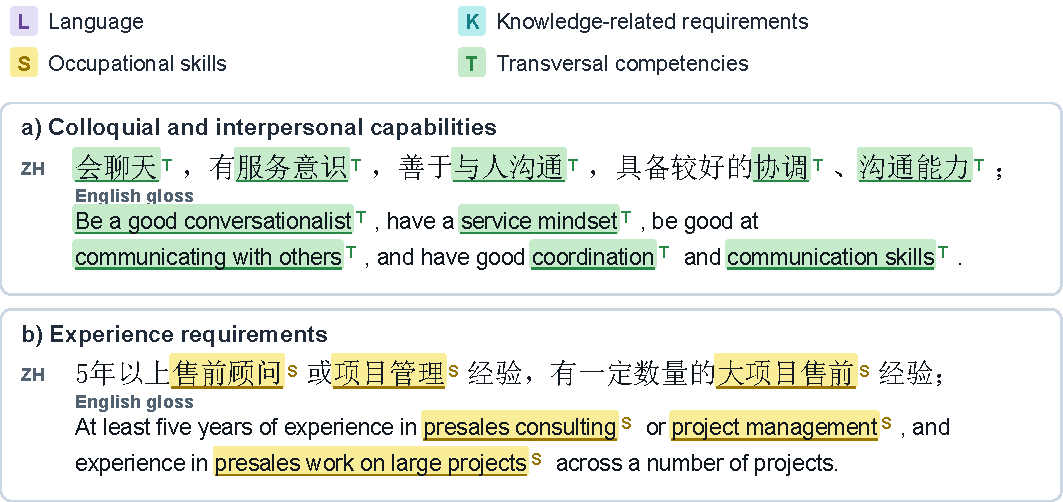
\includegraphics[width=\linewidth]{figures/annotation_examples_additional_20261006.pdf}
\caption{Additional human-reference examples. Chinese highlights retain the frozen reference spans (v4.2.10 metadata); colours and letters align their English glosses. Source IDs and offsets are in the \href{https://github.com/AlfredJamesLi/chinese-skillspan-benchmark/blob/5c12ecd06e37091d8b28a3831738efd1401abdb2/reproduction/manuscript_revision_20261002/source/figures/annotation_examples_corpus_20261003.json}{example metadata}.}
\label{fig:additional-annotation-examples}
\end{figure}
